% 一维波动方程

\pentry{简谐振子\upref{SHO}, 导数与差分\upref{DerDif}, 平面波\upref{PWave}}

\subsection{横波}
我们假设有一根无限长的弦, 质量线密度%未完成:并没有介绍
为 $\lambda$, 弦的\bb{张力}(即拉力)为 $T$, 弦静止时与 $x$ 轴重合. 假设 $t$ 时刻的\bb{波函数}(即弦的形状)为 $y(x, t)$,且弦的振幅较小, 下面我们来求波函数所满足的微分方程, 称为\bb{一维波动方程}.

\begin{figure}[ht]
\centering
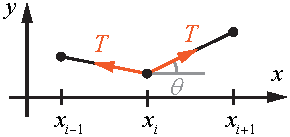
\includegraphics[width=5cm]{./figures/WEq1D1.pdf}
\caption{“微元法” 分析弦的波动} \label{WEq1D_fig1}
\end{figure}

我们用“微元法” 的思想, 把弦划分为许多小线段, 每段长度为 $h$, 质量为 $m_i = \lambda h$, 且质量都集中在左端的端点 $x_i$ 处. 下面我们来考察质点 $m_i$ 的受力情况(\autoref{WEq1D_fig1}). 令 $m_{i+1}$ 对 $m_i$ 的拉力方向与 $x$ 轴夹角为 $\theta$, 由于弦的波动较小, 可以认为 $\theta$ 很小, 这样来自 $m_{i+1}$ 的拉力的两个分量为
\begin{equation}\label{WEq1D_eq1}
\leftgroup{
F_x &= T\cos\theta \approx T\\
F_y &= T\sin\theta \approx T\tan\theta = T\frac{y(x_i+h) -y(x_i)}{h}
}\end{equation}
同理, 来自 $m_{i-1}$ 的拉力的两个分量为
\begin{equation}\label{WEq1D_eq2}
\leftgroup{
F'_x &\approx -T\\
F'_y &\approx T\frac{y(x_i - h) -y(x_i)}{h}
}\end{equation}
把\autoref{WEq1D_eq1} 和\autoref{WEq1D_eq2} 相加, 得 $m_i$ 受 $x$ 方向的合力为零, $y$ 方向的合力为
\begin{equation}
F_y = T\frac{y(x_i+h) - 2y(x_i) + y(x_i-h)}{h}
\end{equation}
结合牛顿定律, 并代入 $m_i = \lambda h$, 有
\begin{equation}
\lambda \pdv[2]{y}{t} = T\frac{y(x_i+h) - 2y(x_i) + y(x_i-h)}{h^2}
\end{equation}
注意到 $h$ 很小, 由\autoref{DerDif_eq5}\upref{DerDif} 可得等式右边为 $T\pdv*[2]{y}{x}$. 于是我们得到波动方程为
\begin{equation}
\pdv[2]{y}{x} - \frac{\lambda}{T}\pdv[2]{y}{t} = 0
\end{equation}

由于这个方程中未知函数 $y(x,t)$ 是一个多元函数, 且出现了偏微分, 我们把它叫做\bb{偏微分方程}.

\subsection{纵波}

\begin{figure}[ht]
\centering
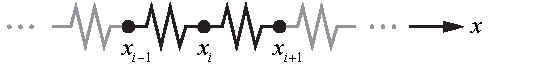
\includegraphics[width=8.3cm]{./figures/WEq1D2.pdf}
\caption{一个常见的纵波模型} \label{WEq1D_fig2}
\end{figure}

以上弦模型中的波动显然是一个横波, 我们也可以建立一个纵波的模型. 如\autoref{WEq1D_fig2}, 我们假设一条无限长的弹簧上的质量都集中于等间距的 $x_i$, 间距为 $h$. 若弹簧的平均线密度为 $\lambda$, 则每个质点的质量为 $m_i = \lambda h$. 为了描述弹簧的弹性, 我们令单位长度弹簧的弹性系数为 $k$, 则长为 $h$ 的一小段弹簧弹性系数为 $k/h$. 若用 $\xi_i$ 来描述 $m_i$ 在 $x$ 方向的位移, 我们可以列出 $m_i$ 的运动方程为
\begin{equation}
\lambda h \pdv[2]{\xi}{t} = F_i = \frac kh [\xi(x_i + h) - 2\xi(x_i) + \xi(x_i - h)]
\end{equation}
同样利用\autoref{DerDif_eq5}\upref{DerDif} 得波动方程为
\begin{equation}
\pdv[2]{\xi}{x} - \frac{\lambda}{k}\pdv[2]{\xi}{t}
\end{equation}

\subsection{方程的解}



